Wikipedia summarizes that SNA  is the process of investigating social structures\cite{wiki_sna}. The structure consists of two parts, individuals and interactions, graphically characterized as nodes and edges in the network. So for the purpose of SNA, we reconfigure the original data as two datasets - the Nodes file and the Edeges file (see Figure \ref{fig:node_file} and \ref{fig:edge_file} for snapshots of the data sets). For each node and edge, we assign type and weight to facilitate our analysis. Details on the categorization and weighting scheme can be found in Appendix \ref{App:AppendixA}.
\begin{figure}[ht]
\caption{Nodes file snapshot}
\label{fig:node_file}
\centering
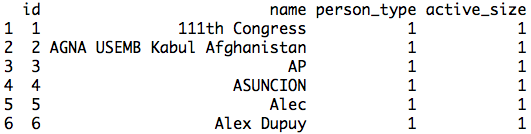
\includegraphics[width=.68\textwidth]{report_node_file}

\caption{Edges file snapshot}
\label{fig:edge_file}
\centering
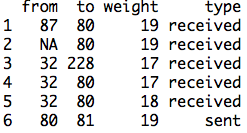
\includegraphics[width=.35\textwidth]{report_edge_file}
\end{figure}
